\subsection{Campo debole}
Si considera la metrica D-dimensionale $g_{\mu\nu}$ nell'approssimazione di campo debole.
Le Vielbein possono essere scritte come \( V^a = (\delta^a_\mu + \frac{1}{2} h^a_\mu) \dx^\mu \): si verifica infatti che, al primo ordine in $|h_{\mu\nu}|$, 
\[ \eta_{ab} V^aV^b = g_{\mu\nu}\dx^\mu \dx^\nu \]
Si verifica immediatamente che 
\[ V^\mu_a = (\delta^\mu_a - \frac{1}{2} h^\mu_a) \]
pertanto si pu\`o usare la formula
\[ \omega_{abc} = V^\mu_a V^\nu_b \partial_\mu V^c_\nu - [cab] + [bca] \]
che, considerando di secondo ordine termini del tipo $(\partial h)h$,  \todo porta al primo ordine a 
\[ \omega_{abc} = \frac{1}{2} [ \partial{[b} h_{c]a} - [abc] + [cab] \]
\[ \omega_{ab} = \frac{1}{2} \partial_{[b} h_{a]c} V^c \]
Siccome si trascurano termini del tipo $(\partial h)(\partial h)$,
\[ R_{ab} = \de \omega_{ab} = -\frac{1}{2} \partial_i \partial_{[a} h_{b]j} V^i \wedge V^j \]

Lo stesso calcolo si pu\`o fare con i simboli di Christoffel:
\[ \Gamma ^\sigma_{\mu\nu} = \frac{1}{2} g^{\rho\sigma}(\partial_\mu g_{\nu\rho} + [\nu\rho\mu] - [\rho\mu\nu]) = \frac{1}{2}(\partial_\mu h^\sigma_\mu + \partial_\nu h^\sigma_\mu - \partial^\sigma h_{\mu\nu} ) \]
e
\[ R_{\mu\nu} = -\partial_{\alpha} \partial_{[\mu} h_{\nu]\beta} \dx^\alpha \dx^\beta \]

Il tensore di Ricci \`e
\[ Ric_{ab} = - \frac{1}{2} \partial^2  h_{ab} + \frac{1}{2} \partial_\nu \partial^\mu h^b_\mu 
              + \frac{1}{2} \partial_\mu \partial^b h^\mu_\nu - \frac{1}{2} \partial_\nu \partial^b h  \]
che con la gauge 
\[ \partial^a \bar{h}_{ab} = 0  \;\;\; ; \;\;\; \bar{h}_{ab} = h_{ab} - \frac{1}{2} \eta_{ab} h \]
diventa
\[ Ric_{ab} = - \frac{1}{2} \partial^2  h_{ab} \]
da cui il tensore di Einstein \`e immediatamente
\[ G_{\mu\nu} = -\frac{1}{2} \partial^2 \bar{h}_{\mu\nu} \]

\todo\todo



\subsection{Funzione di Green}
La funzione di Green del D'Alambertiano, valutata nella sua trasformata di Fourier, risulta essere \( \tilde{G} =- 1/k^2 \). Dovendo integrare questa espressione in $k^0$, si nota subito che ha due poli per \( k^0 = |\vec{k}| \), per cui sar\`a necessaria una prescrizione $i\epsilon$, concretizzata in un cambio di variabile \( k^0 -> k^0 \pm i\epsilon \). La richiesta di causalit\`a permette di fissarne il segno, in quanto corrisponde alla richiesta che la funzione sia nulla per \( x^0 < 0\):  infatti, usando il lemma di Jordan, l'integrale in questo intervallo si annulla chiudendo la circonferenza "sopra" l'asse reale; ma, richiedendo che sia nullo, esso non deve contenere i poli, pertanto si ha una situazione come in \ref{figure:green}.


\begin{figure}[htbp]
 \centering
 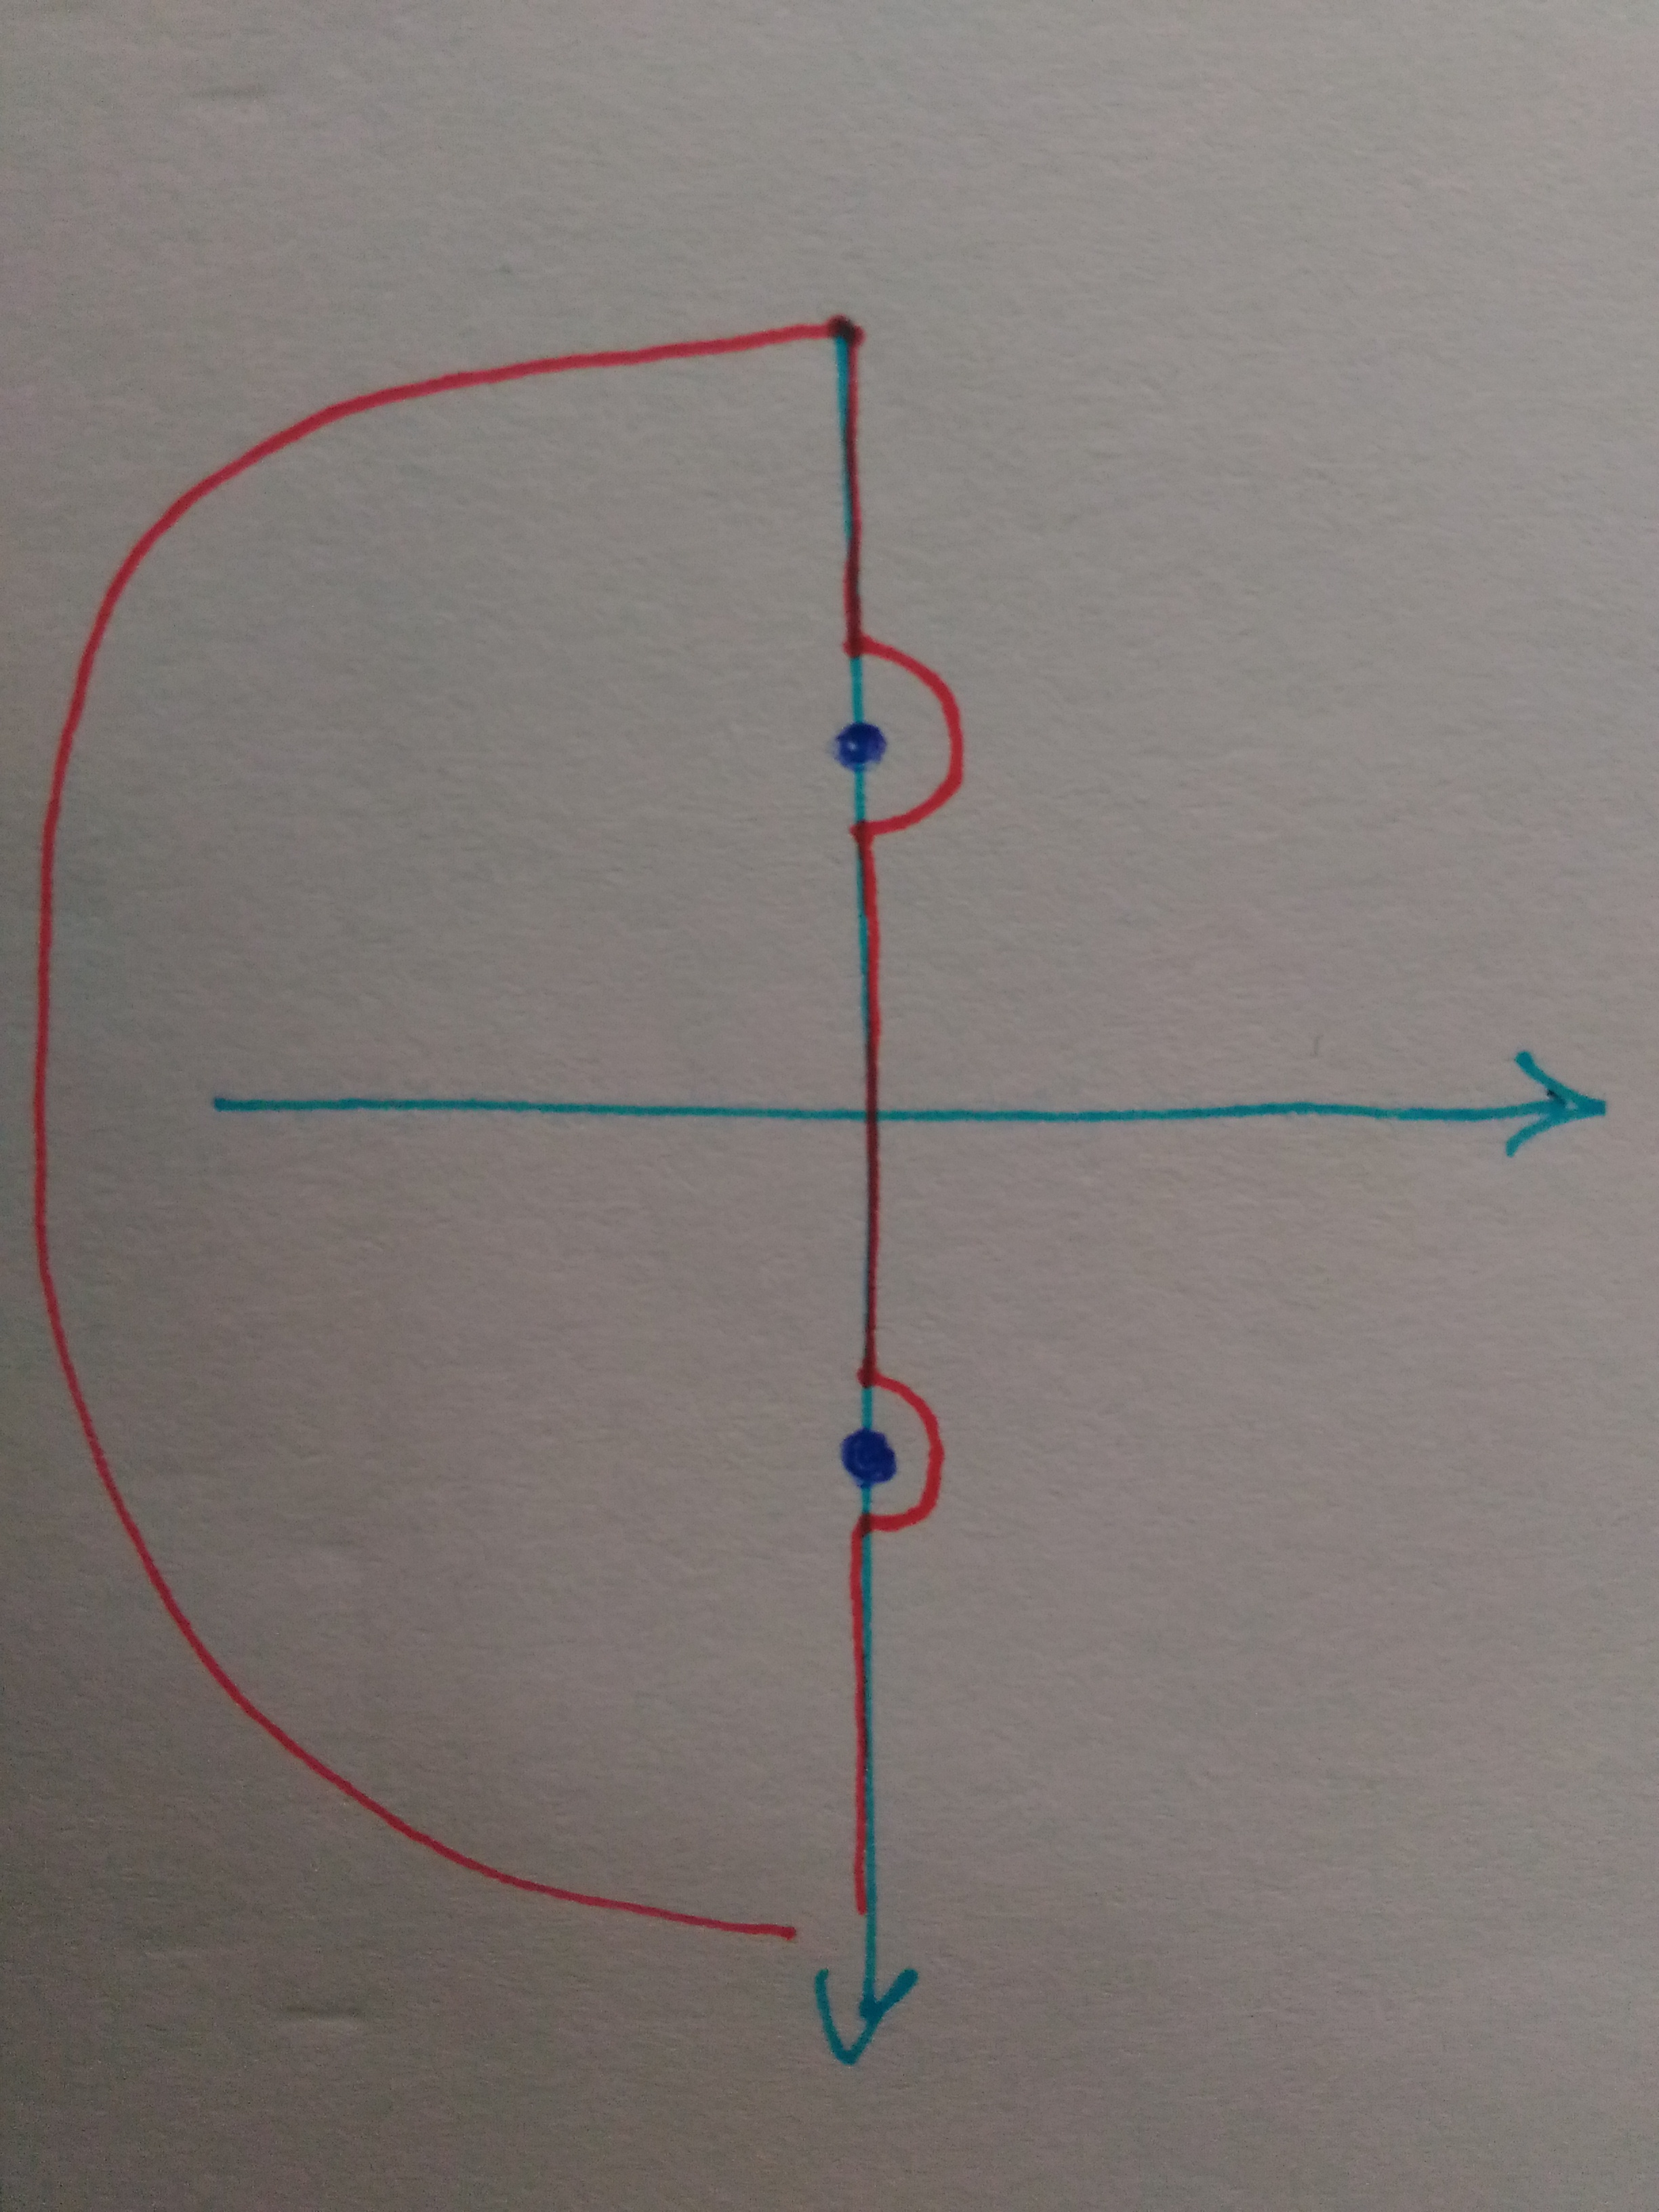
\includegraphics[angle=90, width=\textwidth]{images/foglio5_circuito}
	\caption*{}
 \label{figure:green}
\end{figure}

L'integrale risulta quindi
\[ G_R = \int \frac{\de ^4k}{(2\pi)^4} \frac{e^{ik_\mu x^\mu}}{ (k^0+i\epsilon)^2 - \vec{k}^2 } \]
che diventa col teorema dei residui, in coordinate sferiche
\[ G_R = -\frac{1}{(2\pi)^4} \int \de \phi \; \de \cos\theta \;\de k \;\; k^2 e^{ ik|x|\cos\theta} \frac{2\pi i}{2k} \left[e^{-ikx^0} - e^{ikx^0}\right] \theta(x^0)    \]
